% ============================================================
% Question Bank: ch02-02 Connecting Percents and Proportions
% Topic Title: Connecting Percents and Proportions
% CCSS: 7.RP.A.3
% Questions: 27 (15 MC + 6 SA + 6 Graphical)
% ============================================================

% --- Multiple Choice Questions (15) ---

\begin{practiceQuestion}{2-2-q01}{mc}
\begin{questionText}
Which proportion can be used to find what percent $21$ is of $84$?
\end{questionText}
\choiceA{$\dfrac{21}{84} = \dfrac{p}{100}$}
\choiceB{$\dfrac{84}{21} = \dfrac{p}{100}$}
\choiceC{$\dfrac{p}{21} = \dfrac{84}{100}$}
\choiceD{$\dfrac{21}{p} = \dfrac{84}{100}$}
\correctAnswer{A}
\explanation{Part over whole equals percent over $100$: $\frac{21}{84} = \frac{p}{100}$. Cross-multiply to solve.}
\end{practiceQuestion}

\begin{practiceQuestion}{2-2-q02}{mc}
\begin{questionText}
Use a proportion to find $72\%$ of $350$.
\end{questionText}
\choiceA{$245$}
\choiceB{$250$}
\choiceC{$252$}
\choiceD{$280$}
\correctAnswer{C}
\explanation{Set up: $\frac{n}{350} = \frac{72}{100}$. Cross-multiply: $100n = 25{,}200$. Divide: $n = 252$.}
\end{practiceQuestion}

\begin{practiceQuestion}{2-2-q03}{mc}
\begin{questionText}
In a parking lot, $36$ out of $90$ vehicles are trucks. What percent are trucks?
\end{questionText}
\choiceA{$30\%$}
\choiceB{$36\%$}
\choiceC{$40\%$}
\choiceD{$45\%$}
\correctAnswer{C}
\explanation{$\frac{36}{90} = \frac{p}{100}$. Cross-multiply: $90p = 3{,}600$. Divide: $p = 40\%$.}
\end{practiceQuestion}

\begin{practiceQuestion}{2-2-q04}{mc}
\begin{questionText}
Which proportion shows that $56$ is $80\%$ of some number $w$?
\end{questionText}
\choiceA{$\dfrac{56}{w} = \dfrac{80}{100}$}
\choiceB{$\dfrac{w}{56} = \dfrac{80}{100}$}
\choiceC{$\dfrac{80}{56} = \dfrac{w}{100}$}
\choiceD{$\dfrac{56}{80} = \dfrac{w}{100}$}
\correctAnswer{A}
\explanation{Part ($56$) over whole ($w$) equals percent ($80$) over $100$: $\frac{56}{w} = \frac{80}{100}$.}
\end{practiceQuestion}

\begin{practiceQuestion}{2-2-q05}{mc}
\begin{questionText}
Solve using a proportion: $84$ is $70\%$ of what number?
\end{questionText}
\choiceA{$58.8$}
\choiceB{$100$}
\choiceC{$114$}
\choiceD{$120$}
\correctAnswer{D}
\explanation{$\frac{84}{w} = \frac{70}{100}$. Cross-multiply: $70w = 8{,}400$. Divide: $w = 120$.}
\end{practiceQuestion}

\begin{practiceQuestion}{2-2-q06}{mc}
\begin{questionText}
A theater has $400$ seats. If $85\%$ are filled for a show, how many seats are empty?
\end{questionText}
\choiceA{$40$}
\choiceB{$55$}
\choiceC{$60$}
\choiceD{$85$}
\correctAnswer{C}
\explanation{Filled: $\frac{n}{400} = \frac{85}{100}$ gives $n = 340$. Empty: $400 - 340 = 60$ seats.}
\end{practiceQuestion}

\begin{practiceQuestion}{2-2-q07}{mc}
\begin{questionText}
$45$ out of $300$ students chose basketball as their favorite sport. What percent is that?
\end{questionText}
\choiceA{$12\%$}
\choiceB{$15\%$}
\choiceC{$18\%$}
\choiceD{$45\%$}
\correctAnswer{B}
\explanation{$\frac{45}{300} = \frac{p}{100}$. Cross-multiply: $300p = 4{,}500$. Divide: $p = 15\%$.}
\end{practiceQuestion}

\begin{practiceQuestion}{2-2-q08}{mc}
\begin{questionText}
Which equation is equivalent to the proportion $\dfrac{n}{180} = \dfrac{45}{100}$?
\end{questionText}
\choiceA{$n = 180 \div 45$}
\choiceB{$100n = 180 \times 45$}
\choiceC{$45n = 180 \times 100$}
\choiceD{$n = 45 \times 180$}
\correctAnswer{B}
\explanation{Cross-multiply: $100 \times n = 180 \times 45$, giving $100n = 8{,}100$.}
\end{practiceQuestion}

\begin{practiceQuestion}{2-2-q09}{mc}
\begin{questionText}
Maria solved ``$64$ is what percent of $160$?'' using two methods. With the proportion she got $40\%$. With the equation she divided $64 \div 160 = 0.40 = 40\%$. Which statement is true?
\end{questionText}
\choiceA{Only the proportion method is correct}
\choiceB{Only the equation method is correct}
\choiceC{Both methods give the same correct answer}
\choiceD{Neither method is correct}
\correctAnswer{C}
\explanation{Both approaches are valid: the proportion $\frac{64}{160} = \frac{p}{100}$ and the equation $p = \frac{64}{160} \times 100$ both give $40\%$.}
\end{practiceQuestion}

\begin{practiceQuestion}{2-2-q10}{mc}
\begin{questionText}
$108$ is $135\%$ of what number?
\end{questionText}
\choiceA{$72$}
\choiceB{$80$}
\choiceC{$90$}
\choiceD{$145.8$}
\correctAnswer{B}
\explanation{$\frac{108}{w} = \frac{135}{100}$. Cross-multiply: $135w = 10{,}800$. Divide: $w = 80$.}
\end{practiceQuestion}

\begin{practiceQuestion}{2-2-q11}{mc}
\begin{questionText}
A bakery made $240$ muffins. If $78$ were blueberry, what percent were blueberry?
\end{questionText}
\choiceA{$25\%$}
\choiceB{$30\%$}
\choiceC{$32.5\%$}
\choiceD{$78\%$}
\correctAnswer{C}
\explanation{$\frac{78}{240} = \frac{p}{100}$. Cross-multiply: $240p = 7{,}800$. Divide: $p = 32.5\%$.}
\end{practiceQuestion}

\begin{practiceQuestion}{2-2-q12}{mc}
\begin{questionText}
A camp has $180$ campers. The proportion $\dfrac{n}{180} = \dfrac{65}{100}$ is used to find how many campers signed up for swimming. What is $n$?
\end{questionText}
\choiceA{$65$}
\choiceB{$108$}
\choiceC{$117$}
\choiceD{$120$}
\correctAnswer{C}
\explanation{Cross-multiply: $100n = 180 \times 65 = 11{,}700$. Divide: $n = 117$ campers.}
\end{practiceQuestion}

\begin{practiceQuestion}{2-2-q13}{mc}
\begin{questionText}
A store sold $126$ of its $420$ items last week. What percent of items were sold?
\end{questionText}
\choiceA{$25\%$}
\choiceB{$30\%$}
\choiceC{$33\%$}
\choiceD{$42\%$}
\correctAnswer{B}
\explanation{$\frac{126}{420} = \frac{p}{100}$. Cross-multiply: $420p = 12{,}600$. Divide: $p = 30\%$.}
\end{practiceQuestion}

\begin{practiceQuestion}{2-2-q14}{mc}
\begin{questionText}
Solve: $\dfrac{n}{360} = \dfrac{15}{100}$. What is $n$?
\end{questionText}
\choiceA{$36$}
\choiceB{$45$}
\choiceC{$54$}
\choiceD{$60$}
\correctAnswer{C}
\explanation{Cross-multiply: $100n = 360 \times 15 = 5{,}400$. Divide: $n = 54$.}
\end{practiceQuestion}

\begin{practiceQuestion}{2-2-q15}{mc}
\begin{questionText}
A student sets up the proportion $\dfrac{30}{w} = \dfrac{24}{100}$ and finds $w = 125$. What question was the student answering?
\end{questionText}
\choiceA{What is $24\%$ of $30$?}
\choiceB{$30$ is $24\%$ of what number?}
\choiceC{What percent of $30$ is $24$?}
\choiceD{$24$ is what percent of $30$?}
\correctAnswer{B}
\explanation{The proportion has the part ($30$) over the whole ($w$) equal to $\frac{24}{100}$. This means $30$ is $24\%$ of $w$. Solving: $w = 125$.}
\end{practiceQuestion}

% --- Short Answer Questions (6) ---

\begin{practiceQuestion}{2-2-q16}{sa}
\begin{questionText}
Use a proportion to find $88\%$ of $150$.
\end{questionText}
\correctAnswer{$132$}
\explanation{$\frac{n}{150} = \frac{88}{100}$. Cross-multiply: $100n = 13{,}200$. Divide: $n = 132$.}
\end{practiceQuestion}

\begin{practiceQuestion}{2-2-q17}{sa}
\begin{questionText}
$72$ is what percent of $288$?
\end{questionText}
\correctAnswer{$25\%$}
\explanation{$\frac{72}{288} = \frac{p}{100}$. Cross-multiply: $288p = 7{,}200$. Divide: $p = 25\%$.}
\end{practiceQuestion}

\begin{practiceQuestion}{2-2-q18}{sa}
\begin{questionText}
$117$ is $65\%$ of what number?
\end{questionText}
\correctAnswer{$180$}
\explanation{$\frac{117}{w} = \frac{65}{100}$. Cross-multiply: $65w = 11{,}700$. Divide: $w = 180$.}
\end{practiceQuestion}

\begin{practiceQuestion}{2-2-q19}{sa}
\begin{questionText}
A farm has $240$ animals. $42$ are goats. What percent of the animals are goats?
\end{questionText}
\correctAnswer{$17.5\%$}
\explanation{$\frac{42}{240} = \frac{p}{100}$. Cross-multiply: $240p = 4{,}200$. Divide: $p = 17.5\%$.}
\end{practiceQuestion}

\begin{practiceQuestion}{2-2-q20}{sa}
\begin{questionText}
A library goal is to check out $500$ books this month. So far $440$ have been checked out. What percent of the goal is that?
\end{questionText}
\correctAnswer{$88\%$}
\explanation{$\frac{440}{500} = \frac{p}{100}$. Cross-multiply: $500p = 44{,}000$. Divide: $p = 88\%$.}
\end{practiceQuestion}

\begin{practiceQuestion}{2-2-q21}{sa}
\begin{questionText}
Solve: $\dfrac{n}{560} = \dfrac{35}{100}$.
\end{questionText}
\correctAnswer{$196$}
\explanation{Cross-multiply: $100n = 560 \times 35 = 19{,}600$. Divide: $n = 196$.}
\end{practiceQuestion}

% --- Graphical Questions (3 GMC + 3 GSA) ---

\begin{practiceQuestion}{2-2-q22}{gmc}
\begin{questionText}
The double number line below shows a percent relationship. What number belongs at the question mark?

\begin{center}
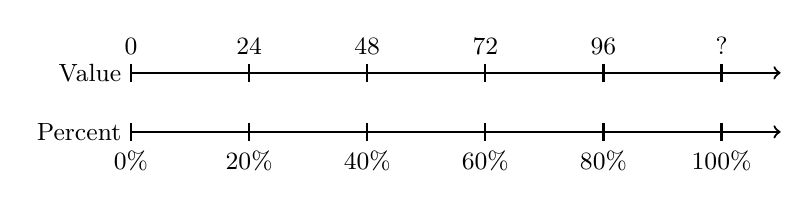
\begin{tikzpicture}[scale=0.75]
  \draw[thick,->] (0,1) -- (11,1);
  \node[left,font=\small] at (0,1) {Value};
  \foreach \x/\lab in {0/0, 2/24, 4/48, 6/72, 8/96, 10/?} {
    \draw[thick] (\x,0.85) -- (\x,1.15);
    \node[above,font=\small] at (\x,1.15) {\lab};
  }
  \draw[thick,->] (0,0) -- (11,0);
  \node[left,font=\small] at (0,0) {Percent};
  \foreach \x/\lab in {0/0\%, 2/20\%, 4/40\%, 6/60\%, 8/80\%, 10/100\%} {
    \draw[thick] (\x,-0.15) -- (\x,0.15);
    \node[below,font=\small] at (\x,-0.15) {\lab};
  }
\end{tikzpicture}
\end{center}
\end{questionText}
\choiceA{$100$}
\choiceB{$108$}
\choiceC{$112$}
\choiceD{$120$}
\correctAnswer{D}
\explanation{Each $20\%$ corresponds to $24$. At $100\%$: $24 \times 5 = 120$. Alternatively, if $20\%$ is $24$, the whole is $24 \div 0.20 = 120$.}
\end{practiceQuestion}

\begin{practiceQuestion}{2-2-q23}{gmc}
\begin{questionText}
The bar model below is divided into $5$ equal sections. The total value is $160$. What percent of the total does the shaded part represent?

\begin{center}
\begin{tikzpicture}[scale=0.6]
  \foreach \i in {0,...,4} {
    \draw[thick] (\i*1.6,0) rectangle (\i*1.6+1.6,0.8);
  }
  \fill[funGreen!40] (0,0) rectangle (1.6,0.8);
  \fill[funGreen!40] (1.6,0) rectangle (3.2,0.8);
  \fill[funGreen!40] (3.2,0) rectangle (4.8,0.8);
  \foreach \i in {0,...,4} {
    \draw[thick] (\i*1.6,0) rectangle (\i*1.6+1.6,0.8);
  }
  \node[above,font=\small] at (2.4,0.8) {Shaded};
  \draw[thick,<->] (0,-0.5) -- (8,-0.5) node[midway,below,font=\small] {Total $= 160$};
\end{tikzpicture}
\end{center}
\end{questionText}
\choiceA{$30\%$}
\choiceB{$40\%$}
\choiceC{$50\%$}
\choiceD{$60\%$}
\correctAnswer{D}
\explanation{$3$ out of $5$ sections are shaded: $\frac{3}{5} = \frac{p}{100}$. Cross-multiply: $5p = 300$, so $p = 60\%$.}
\end{practiceQuestion}

\begin{practiceQuestion}{2-2-q24}{gmc}
\begin{questionText}
The table below shows the number of students in each elective. What percent of the students are in Art?

\begin{center}
\begin{tabular}{|l|c|}
\hline
\textbf{Elective} & \textbf{Students} \\
\hline
Art & $27$ \\
\hline
Music & $18$ \\
\hline
Drama & $9$ \\
\hline
Coding & $36$ \\
\hline
\end{tabular}
\end{center}
\end{questionText}
\choiceA{$20\%$}
\choiceB{$27\%$}
\choiceC{$30\%$}
\choiceD{$36\%$}
\correctAnswer{C}
\explanation{Total: $27 + 18 + 9 + 36 = 90$. Art: $\frac{27}{90} = \frac{p}{100}$. Cross-multiply: $90p = 2{,}700$, so $p = 30\%$.}
\end{practiceQuestion}

\begin{practiceQuestion}{2-2-q25}{gsa}
\begin{questionText}
The proportion model below shows two bars. Find the value of $n$.

\begin{center}
\begin{tikzpicture}[scale=0.6]
  \draw[thick] (0,1.5) rectangle (8,2.3);
  \fill[funBlue!40] (0,1.5) rectangle (5.6,2.3);
  \draw[thick] (0,1.5) rectangle (8,2.3);
  \draw[thick] (5.6,1.5) -- (5.6,2.3);
  \node[above,font=\small] at (2.8,2.3) {$n$};
  \node[right,font=\small] at (8.2,1.9) {$200$};
  \draw[thick] (0,0) rectangle (10,0.8);
  \fill[funBlue!40] (0,0) rectangle (7,0.8);
  \draw[thick] (0,0) rectangle (10,0.8);
  \draw[thick] (7,0) -- (7,0.8);
  \node[below,font=\small] at (3.5,0) {$70$};
  \node[right,font=\small] at (10.2,0.4) {$100$};
\end{tikzpicture}
\end{center}
\end{questionText}
\correctAnswer{$140$}
\explanation{$\frac{n}{200} = \frac{70}{100}$. Cross-multiply: $100n = 14{,}000$. Divide: $n = 140$.}
\end{practiceQuestion}

\begin{practiceQuestion}{2-2-q26}{gsa}
\begin{questionText}
Use the table to answer: a factory produces the items shown below. What percent of all items are medium?

\begin{center}
\begin{tabular}{|l|c|}
\hline
\textbf{Size} & \textbf{Quantity} \\
\hline
Small & $54$ \\
\hline
Medium & $108$ \\
\hline
Large & $78$ \\
\hline
X-Large & $60$ \\
\hline
\end{tabular}
\end{center}
\end{questionText}
\correctAnswer{$36\%$}
\explanation{Total items: $54 + 108 + 78 + 60 = 300$. Medium: $\frac{108}{300} = \frac{p}{100}$. Cross-multiply: $300p = 10{,}800$, so $p = 36\%$.}
\end{practiceQuestion}

\begin{practiceQuestion}{2-2-q27}{gsa}
\begin{questionText}
The number line below shows that the shaded region represents $45\%$ of the whole. If the shaded region has a value of $63$, what is the value of the whole?

\begin{center}
\begin{tikzpicture}[scale=0.7]
  \draw[thick] (0,0) -- (10,0);
  \draw[thick] (0,-0.2) -- (0,0.2) node[above,font=\small] {$0$};
  \draw[thick] (4.5,-0.2) -- (4.5,0.2) node[above,font=\small] {$63$};
  \draw[thick] (10,-0.2) -- (10,0.2) node[above,font=\small] {?};
  \fill[funBlue!30] (0,-0.1) rectangle (4.5,0.1);
  \node[below,font=\small] at (2.25,-0.3) {$45\%$};
  \node[below,font=\small] at (7.25,-0.3) {$55\%$};
\end{tikzpicture}
\end{center}
\end{questionText}
\correctAnswer{$140$}
\explanation{$\frac{63}{w} = \frac{45}{100}$. Cross-multiply: $45w = 6{,}300$. Divide: $w = 140$.}
\end{practiceQuestion}
